%%%%%%%%%%%%%%%%%%%%%%%%%%%%%%%%%%%%%%%%%%%%%%%%%%%%%%%%%%%%%%%%%%%%%%%%%%%%%
% Баталов Семен, 2021                                                       %
%%%%%%%%%%%%%%%%%%%%%%%%%%%%%%%%%%%%%%%%%%%%%%%%%%%%%%%%%%%%%%%%%%%%%%%%%%%%%

\documentclass[12pt, a4paper]{article}
\usepackage[left=2.5cm, right=2.5cm, top=2.5cm, bottom=2.5cm]{geometry}
\usepackage[utf8]{inputenc}
\usepackage{graphicx}
\graphicspath{{./pictures/}}
\usepackage[english, russian]{babel}
\usepackage{indentfirst}
\usepackage{misccorr}
\usepackage{amsmath}

\title{Аппроксимация многомерной функции перцептроном с двумя скрытыми слоями.}
\author{Баталов Семен}
\date{02.03.2021}

\begin{document}
    
    \sloppy
    
    \maketitle
    
    \section{Перцептрон}
    
    Для аппроксимации любой непрерывной вектор-функции достаточно 
    использовать перцептрон с двумя скрытыми слоями. Это следует из теоремы 
    Колмогорова.
    
    При решении поставленной задачи использовался перцептрон с 2000 
    нейронами в первом и 40 нейронами во втором внутренних слоях (количесво 
    нейронов во входном и выходном слоях варьировалось в зависимости от вида 
    аппроксимируемой функции). В качестве активационной функции 
    использовалась функция <<\textbf{RELU}>>. В качестве функции ошибки 
    использовалась <<\textbf{MAE}>> (Mean Absolute Error). Количество эпох 
    при обучении составило 60.
    
    \section{Обучение и оценка}
    
    Сначала производилась подготовка данных для обучения. Она заключалась в 
    создании в области определения функции сетки, размерность которой 
    совпадала с размерностью области определения, далее в узлах сетки 
    расчитывались значения этой функции. Таким образом, получался датасет 
    для обучения, то есть координаты узлов~--~входные данные, значения 
    функции в них~--~выходные.
    
    Далее из датасета случайно извлекалась обучающая и тестировочная 
    выборки. Оценкой качества работы перцептрона был результат, возвращаемый 
    функцией <<\textbf{MAE}>>, примененной к тестировочной выборке. Для 
    наглядности были также построены графики (и их приближения) некоторых 
    одномерных функций.
    
    \section{Инструменты}
    
    Языком разработки был <<\textbf{Python}>>. Для работы с нейросетью 
    использовалась подбиблиотека <<\textbf{Keras}>> библиотеки 
    <<\textbf{TensorFlow}>>. Также для разделения датасета на обучающую и 
    тестировочную выборки использовалась библиотека <<\textbf{Sklearn}>>. 
    Подробнее о программе можно узнать в папке <<\textbf{source}>> проекта.
    
    \section{Эксперименты и результаты}
    
    Здесь приведено описание некоторых функций, на которых проверялась 
    корректность работы программы. Также изображены графики некоторых из них и приближенно вычисленные значения.
    
    \subsection{$f(x) = - x^2 + 5$}
    
    Непрерывная одномерная функция. Область аппроксимации:~$[-1, 1]$; шаг 
    сетки:~$0.01$; размер обучающей выборки: $0.6~-~0.8$.
    
    Величина ошибки (MAE): 0.009~-~0.085.
    
    \subsection{$f(x) = sin(x) + 1$}
    
    Непрерывная одномерная функция. Область аппроксимации:~$[0, 6.5]$; шаг сетки:~$0.01$; размер обучающей выборки: $0.6~-~0.8$.
    
    Величина ошибки (MAE): 0.021~-~0.100.
    
    \subsection{$f(x) = \sqrt{x}$}
    
    Непрерывная одномерная функция. Область аппроксимации:~$[0, 6.5]$; шаг сетки:~$0.01$; размер обучающей выборки: $0.6~-~0.8$.
    
    Величина ошибки (MAE): 0.006~-~0.015.
    
    \subsection{$f(x, y) = x + y$}
    
    Непрерывная функция двух переменных. Область аппроксимации:~$[0, 2] \times [0, 2]$; шаг сетки:~$0.1$; размер обучающей выборки: $0.6~-~0.8$.
    
    Величина ошибки (MAE): 0.007~-~0.05.
    
    \subsection{$f(x, y) = (x + y, x^2 \cdot y)$}
    
    Непрерывная функция двух переменных. Область аппроксимации:~$[0, 2] \times [0, 2]$; шаг сетки:~$0.1$; размер обучающей выборки: $0.6~-~0.8$.
    
    Величина ошибки (MAE): 0.029~-~0.036.
    
    \begin{figure}[h]
        \center
        \begin{tabular}{cc}
            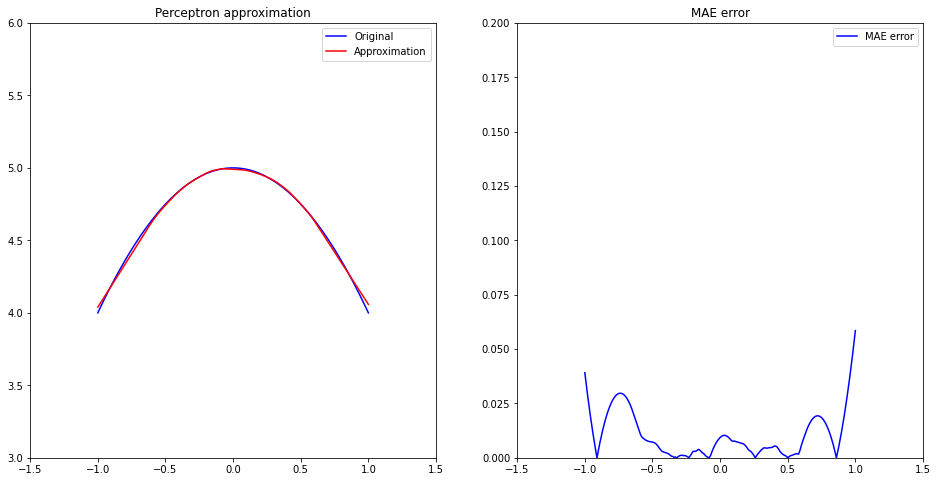
\includegraphics[width = 7cm]{f11_1_1.png}
            &
            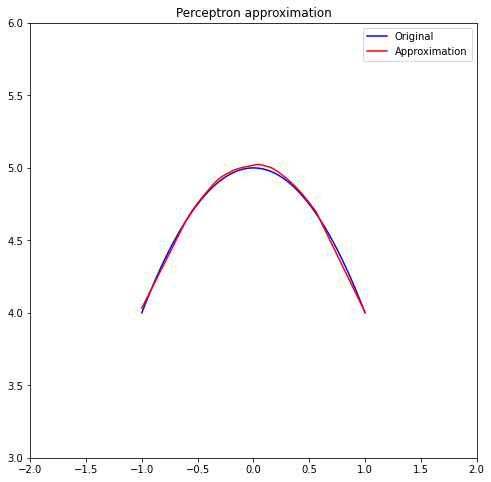
\includegraphics[width = 7cm]{f11_1_2.png} \\
            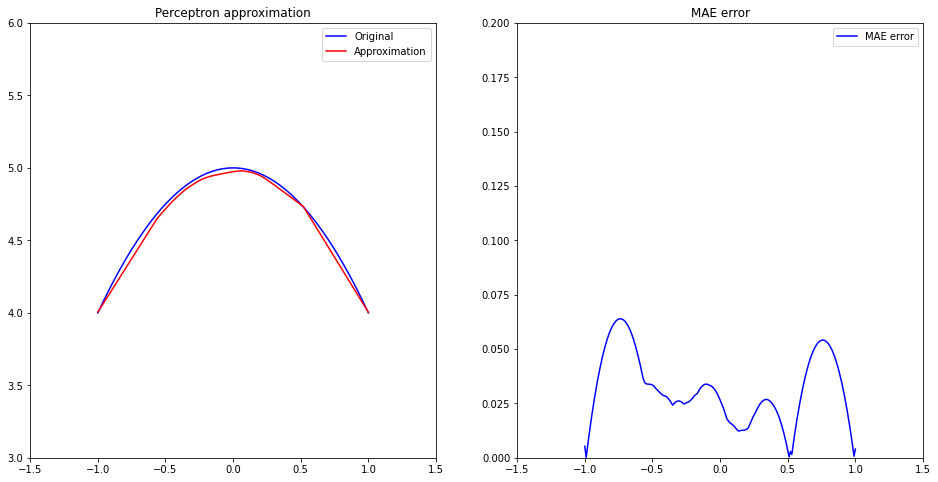
\includegraphics[width = 7cm]{f11_1_3.png}
            &
            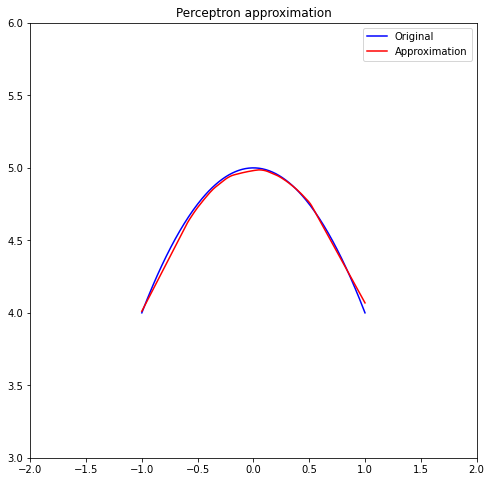
\includegraphics[width = 7cm]{f11_1_4.png} \\
        \end{tabular}
        \label{image1}
        \caption{Аппроксимация функции $f(x) = - x^2 + 5$.}
    \end{figure}
    
    \begin{figure}[h]
        \center
        \begin{tabular}{cc}
            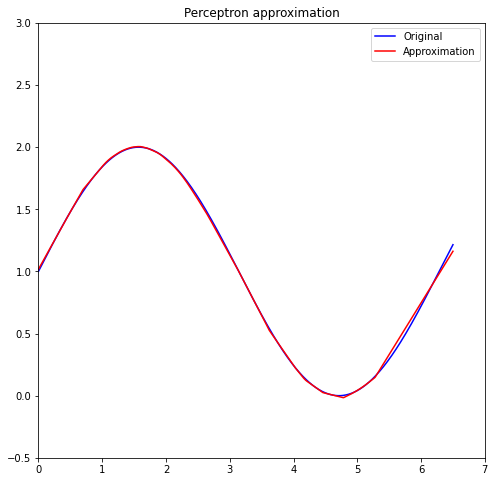
\includegraphics[width = 7cm]{f11_2_1.png}
            &
            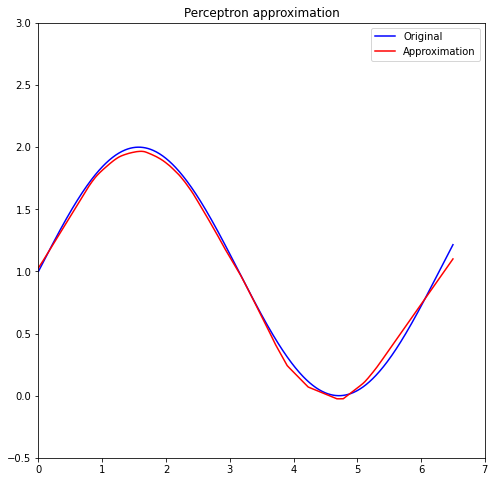
\includegraphics[width = 7cm]{f11_2_2.png} \\
            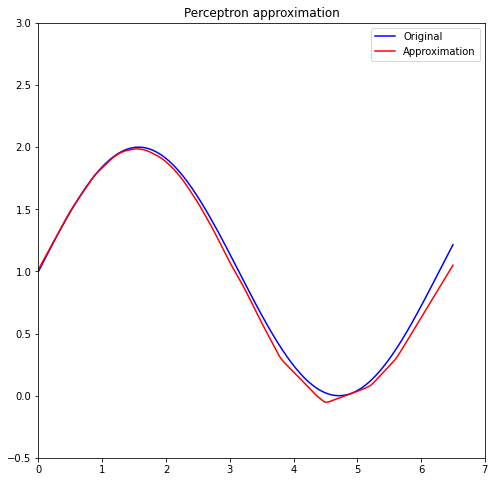
\includegraphics[width = 7cm]{f11_2_3.png}
            &
            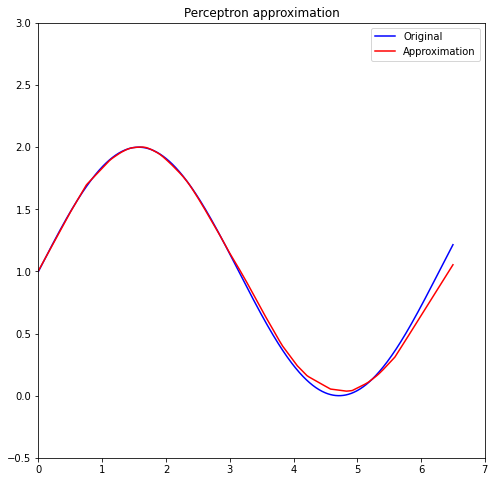
\includegraphics[width = 7cm]{f11_2_4.png} \\
        \end{tabular}
        \label{image2}
        \caption{Аппроксимация функции $f(x) = sin(x) + 1$.}
    \end{figure}
    
    \begin{figure}[h]
        \center
        \begin{tabular}{cc}
            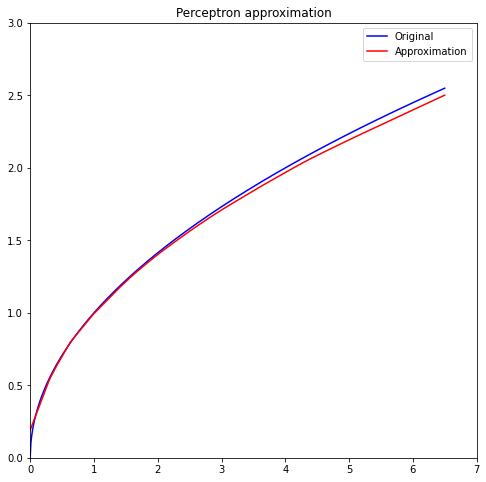
\includegraphics[width = 7cm]{f11_3_1.png}
            &
            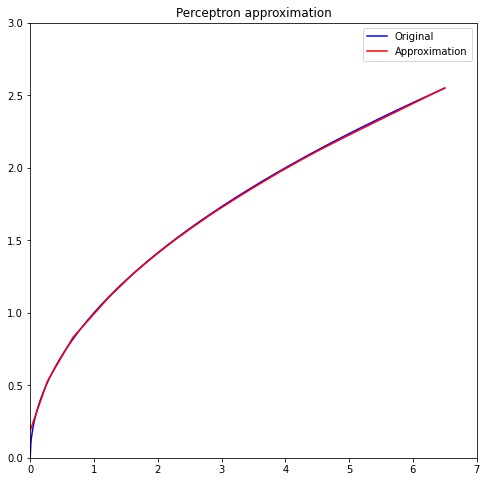
\includegraphics[width = 7cm]{f11_3_2.png} \\
            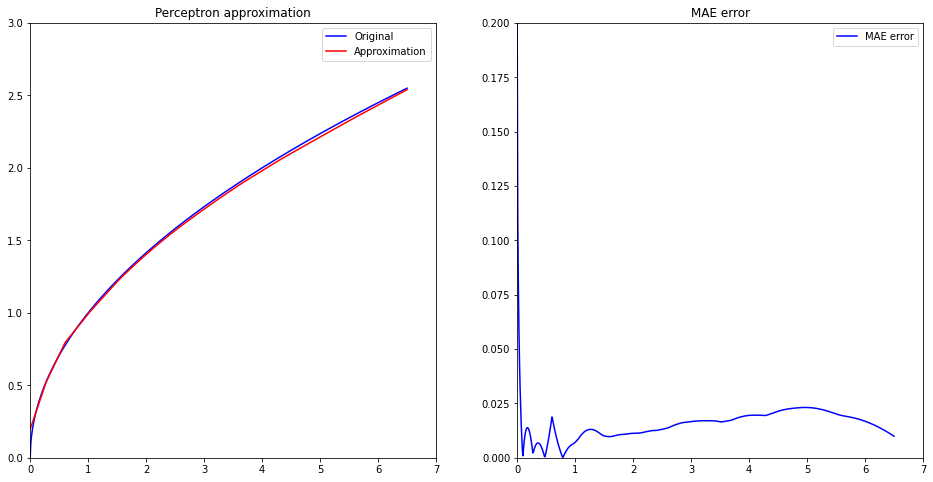
\includegraphics[width = 7cm]{f11_3_3.png}
            &
            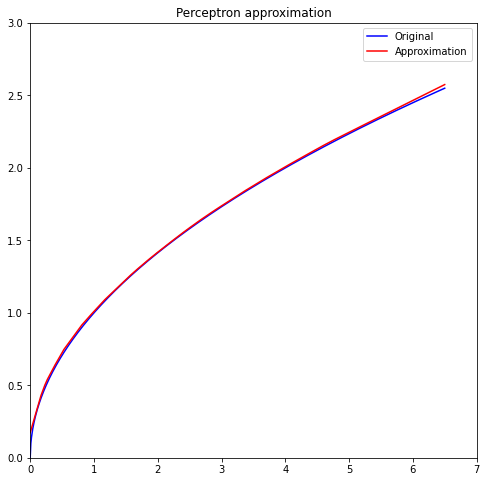
\includegraphics[width = 7cm]{f11_3_4.png} \\
        \end{tabular}
        \label{image3}
        \caption{Аппроксимация функции $f(x) = \sqrt{x}$.}
    \end{figure}
    
\end{document}